%; whizzy paragraph -pdf xpdf -latex ./whizzypdfptex.sh
%; whizzy-paragraph "^\\\\begin{frame}"
% latex beamer presentation.
% platex, latex-beamer $B$G%3%s%Q%$%k$9$k$3$H$rA[Dj!#(B 

%     Tokyo Debian Meeting resources
%     Copyright (C) 2009 Junichi Uekawa
%     Copyright (C) 2009 Nobuhiro Iwamatsu

%     This program is free software; you can redistribute it and/or modify
%     it under the terms of the GNU General Public License as published by
%     the Free Software Foundation; either version 2 of the License, or
%     (at your option) any later version.

%     This program is distributed in the hope that it will be useful,
%     but WITHOUT ANY WARRANTY; without even the implied warreanty of
%     MERCHANTABILITY or FITNESS FOR A PARTICULAR PURPOSE.  See the
%     GNU General Public License for more details.

%     You should have received a copy of the GNU General Public License
%     along with this program; if not, write to the Free Software
%     Foundation, Inc., 51 Franklin St, Fifth Floor, Boston, MA  02110-1301 USA

\documentclass[cjk,dvipdfm,12pt]{beamer}
\usetheme{Tokyo}
\usepackage{monthlypresentation}

%  preview (shell-command (concat "evince " (replace-regexp-in-string "tex$" "pdf"(buffer-file-name)) "&")) 
%  presentation (shell-command (concat "xpdf -fullscreen " (replace-regexp-in-string "tex$" "pdf"(buffer-file-name)) "&"))
%  presentation (shell-command (concat "evince " (replace-regexp-in-string "tex$" "pdf"(buffer-file-name)) "&"))

%http://www.naney.org/diki/dk/hyperref.html
%$BF|K\8l(BEUC$B7O4D6-$N;~(B
\AtBeginDvi{\special{pdf:tounicode EUC-UCS2}}
%$B%7%U%H(BJIS$B7O4D6-$N;~(B
%\AtBeginDvi{\special{pdf:tounicode 90ms-RKSJ-UCS2}}

\title{$BEl5~%(%j%"(BDebian$BJY6/2q(B}
\subtitle{$BBh(B75$B2s(B 2011$BG/(B5$B7nEY(B}
\author{$B4d>>(B $B?.MN(B iwamatsu@debian.org\\IRC nick: iwamatsu}
\date{2011$BG/(B5$B7n(B21$BF|(B}
\logo{
\includegraphics[width=8cm]{image200607/openlogo-light.eps}}

\begin{document}

\frame{\titlepage{}}

\section{}
\begin{frame}
 \frametitle{Agenda}
\begin{minipage}[t]{0.45\hsize}
  \begin{itemize}
  \item $BCm0U;v9`(B
	\begin{itemize}
	 \item $B0{<r6X;_(B
	 \item $B=!656X;_(B
	 \item $B1DMx3hF06X;_(B
	\end{itemize}
   \item $B:G6a$"$C$?(BDebian$B4XO"$N%$%Y%s%HJs9p(B
	\begin{itemize}
	 \item $BBh(B75$B2s(B $BEl5~%(%j%"(B Debian$BJY6/2q(B
         \item $BBh(B 46 $B2s4X@>(B Debian $BJY6/2q(B@OSC2011 Kobe
	\end{itemize}
 \end{itemize}
\end{minipage} 
\begin{minipage}[t]{0.45\hsize}
 \begin{itemize}
  \item Apache2 $B$N%b%8%e!<%k$r$D$/$C$F$_$?(B
  \item Debian on NiftyCloud
  \item Debian/m68k $B3+H/(B
  \item $B7n4)(BPPC64$B%]!<%F%#%s%0(B
 \end{itemize}
\end{minipage}
\end{frame}

\begin{frame}
 \frametitle{$BA02s(B}
\begin{minipage}[t]{0.45\hsize}
  \begin{itemize}
  \item $BCm0U;v9`(B
	\begin{itemize}
	 \item $B0{?)6X;_(B
	 \item $B=!656X;_(B
	 \item $B1DMx3hF06X;_(B
	\end{itemize}
  \end{itemize}
\end{minipage}
\begin{minipage}[t]{0.45\hsize}
\begin{itemize}
  \item $B:G6a$"$C$?(BDebian$B4XO"$N%$%Y%s%HJs9p(B
 \begin{itemize}
  \item $B2qD9="G$0';"(B
  \item backports.debian.org$B$NOC(B
  \item initramfs-tools$B$NOC(B
  \item $B7n4)(BPPC64$B%]!<%F%#%s%0(B
  \item $BKM$,(BDD$BL\;X$9$N<jEA$C$F$/$@$5$$(B
 \end{itemize}
 \end{itemize}
\end{minipage}
\end{frame}


\emtext{$B%$%Y%s%HJs9p(B}

\emtext{DWN quiz}

\section{DWN quiz}
\begin{frame}{Debian $B>o<1%/%$%:(B}

Debian $B$N>o<1!"$b$A$m$sCN$C$F$^$9$h$M(B?
$BCN$i$J$$$J$s$FCQ$:$+$7$/$F!"CN$i$J$$$H$O8@$($J$$$"$s$J$3$H$d$3$s$J$3$H!"(B
$B$_$s$J$G3NG'$7$F$_$^$7$g$&!#(B

$B:#2s$N=PBjHO0O$O(B\url{debian-devel-announce@lists.deban.org} $B$KEj9F$5$l$?(B
$BFbMF$H(BDebian Project News$B$+$i$G$9!#(B

\end{frame}

\subsection{$BLdBj(B}
%; whizzy-master ../debianmeetingresume201101.tex
% $B0J>e$N@_Dj$r$7$F$$$k$?$a!"$3$N%U%!%$%k$G(B M-x whizzytex $B$9$k$H!"(Bwhizzytex$B$,MxMQ$G$-$^$9!#(B
%
% $B$A$J$_$K!"%/%$%:$OJL%V%i%s%A$G:n@.$7!"$N$A$K%^!<%8$7$^$9!#5U$K%^!<%8$7(B
% $B$J$$$h$&$K$7$^$7$g$&!#(B
% (shell-command "git checkout quiz-prepare")

\santaku
{HPPA $B$H(B alpha $B$N0\E>@h$O$I$3$G$7$g$&$+!)(B}
{buildd.debian.or.jp}
{buildd.debian-ports.org}
{www.buildd.net}
{B}
{}

\santaku
{linux$B%+!<%M%k(B 2.6.39$B$,(BDebian$B$KF~$k$3$H$K$h$C$F5/$-$kJQ99$O!)(B}
{i386-bigmem$B$,(Bi386-pae$B$K$J$C$?(B}
{amd64$B$,(Bi386$B$K$J$C$?(B}
{i386$B$O(Bamd64$B$N%^%k%A%P%$%J%j$K$J$C$?(B}
{A}
{}

\santaku
{Qt3$B%Q%C%1!<%8$,:o=|$5$l$J$$M}M3$O!)(B}
{Qt3$B%f!<%6$K$h$k0%4j$N$?$a(B}
{LSB 4.1$B$,(BQt3$B$rI,MW$H$7$F$$$k$?$a(B}
{$B:o=|$N;EJ}$,$o$+$i$J$$(B}
{B}
{}

\santaku
{Debian$B$N%5!<%P$KDI2C$5$l$?5!G=$O!)(B}
{$B%m%0%$%s$7$F$$$k%f!<%6$r(BIRC$B$KN.$95!G=(B}
{RFC1149 $B$N<BAu(B}
{DNSSEC}
{C}
{}


\emtext{prework}

{\footnotesize
 %; whizzy-master ../debianmeetingresume201101.tex
% $B0J>e$N@_Dj$r$7$F$$$k$?$a!"$3$N%U%!%$%k$G(B M-x whizzytex $B$9$k$H!"(Bwhizzytex$B$,MxMQ$G$-$^$9!#(B



\begin{prework}{ $B%-%?%O%i(B }

Debian$B8BDj$@$H;W$$$D$+$J$$!&!&!&!#(B
($B$*Bj$N0U?^$rFI$_0c$($F$$$k$N$+$b(B)
apt-get$B$r(Bhttp$B$G<B9T$9$k$H%&%'%V%5!<%S%9$H8@$($k(B?
\end{prework}

\begin{prework}{ MATOHARA }

Debian$B;H$$$H$7$F%&%'%V%5!<%S%9$K4|BT$9$k$3$H!%(B
$B:G6a$O>/$J$/$J$j$^$7$?$,!$(BIE $BI,?\$N%5!<%S%9Ey$N4D6-0MB8$N%5!<%S%9$r$d$a(B
 $B$FM_$7$$$G$9!%(B
$B:G6a$@$H(BSilverlight $BI,?\$N%5!<%S%9$G(BMoonlight $B$GF0$-$=$&$GF0$+$J$$$H$$$C(B
 $B$?$3$H$,$"$j$^$7$?!%(B
\url{http://live6.channel.ne.jp/world_ipv6/}
\end{prework}

\begin{prework}{ taitioooo }

$B>pJs$KBP$9$k2]6b$,$J$/$J$k$3$H!#(B

\end{prework}

\begin{prework}{ $BLnEg!!5.1Q(B }

\begin{itemize}
\item jslinux$B$H$$$&6/NO$J%(%_%e%l!<%?$b=P$?$N$G!"%V%i%&%6$GF0$/(BDebian
 experimental$B4D6-$H$+%V%i%&%6$GF0$/(BGnome$B$N$*;n$74D6-$H$+$rDs6!$9$k%&%'%V(B
 $B%5!<%S%9$H$+AGE($+$b!#(B
$B$3$b$-$C$H%&%'%V%5!<%S%9!*!J$J$s$+6u5$FI$a$F$J$$2sEz$J5$$b$9$k$1$I(B...)

\item USB$B$K=q$-9~$a$P(Bdebian$B4D6-$,$=$N$^$^%V!<%H$G$-$k$h$&$J%$%a!<%8$r$D$/$C$F(B
 $B$/$l$k%&%'%V%5!<%S%9$,NI$5$=$&$J5$$b(B...$BNc$($P!"%Q%C%1!<%80lMw$K%A%'%C%/(B
 $BF~$l$F!"(Bsid$B$H$+$K%A%'%C%/F~$l$k$H!"(BUSB$B%a%b%j$K$=$N$^$^=q$-9~$a$P$=$N;E(B
 $BMM$G(Bdebian sid$B$,%V!<%H$G$-$k$h$&$J%+%9%?%`%$%a!<%8$r:n$C$F$/$l$k$H$+!#(B

\item $B%A%'%C%/%\%C%/%9$H%;%l%/%?$@$1$G!"(Bpreceed$B%U%!%$%k@8@.$7$F$/$l$k%&%'%V%5!<(B
 $B%S%9$b$$$$$+$b(B...$BBgNL$N%$%s%9%H!<%k;~$H$+$h$5$=$&!#(B
$B!J$b$&8@$$$?$$J|Bj$G$9$M(B...)
\end{itemize}











\end{prework}

\begin{prework}{ $B4d>>(B $B?.MN(B }
\begin{itemize}
\item $BA4@$3&$N(BWeb$B%5!<%P$rDs6!$9$k(BOS$B$,(BDebian$B$K$J$k$3$H!#(B
\item $BJ,;6%3%s%Q%$%k%5!<%P$H$+M_$7$$!#(B
\end{itemize}


\end{prework}

\begin{prework}{ $BF|HfLn(B $B7<(B }

Web$B%5!<%S%9$b$G$-$l$P5!3#=hM}$7$d$9$$$b$N$,NI$$!#(B
$B$"$H!"%/%i%&%I>e$G$N(BAPI$B$rDs6!$7$F$$$k$h$&$J%5!<%S%9$K!"4X?t7?8@8l$KBP$9(B
 $B$k%5%]!<%H$,A}$($F$[$7$$!#(B

\end{prework}

\begin{prework}{ dictoss($B?yK\!!E5=<(B) }

CPU$B$H$"$k(Bdeb$B%Q%C%1!<%8$rA*Br$9$k$H!"$=$N(BCPU$B8~$1$K:GBg8B$N:GE,2=$7$?%Q%C(B
 $B%1!<%8$H0MB8$9$k%Q%C%1!<%8$r:F%S%k%I$7$F$/$l$k%5!<%S%9!#(B
\end{prework}

\begin{prework}{ kazken3 }

$BK]Lu$r$?$^$K$7$F$$$k$N$G!"%G%#%9%H%j%S%e!<%7%g%s4V2#$I$*$7$G$NK]Lu4XO">p(B
 $BJs$rDs6!$9$k%5%$%H$,$"$l$P$$$$$J$H;W$&$3$H$,$"$j$^$9!#(B

$B!t2]Bj$H$O>/$7%:%l$F$$$k$+$bCN$l$^$;$s$,!"(B
$B!t8D?M8~$1$N%&%'%V%5!<%S%9$K$O?)=}5$L#$H$$$&$H$3$m$b$"$k$N$G!#(B


\end{prework}

\begin{prework}{ $B$^$($@$3$&$X$$(B }

Debian$B%7%9%F%`$G:n$C$?4D6-$H$NAj8_8_49@-!#(B
$BNc$($P!":G6a(BGAE/Python$B$r$h$/;H$&$N$G!":n$C$?%7%9%F%`$r(B
 GAE/Python <-> $B"*(BDebian$B%7%9%F%`$N$I$A$i$G$b(B($B$[$H$s$IJQ99$J$7$G(B)$BF0$+$;$k$H(B
 $BJXMx$G$9$M!#(B
$B$9$0;O$a$k$N$K%/%i%&%I%5!<%S%9$rMxMQ$7$F:n$C$?$1$I>-Mh$O(BDebian$B$GF0$+$7$?(B
 $B$$!"5U$K:#$O@/<#E*$JM}M3$G30$K=P$;$J$$(BDebian$B%7%9%F%`$r>-Mh$O<+J,$N4IM}(B
 $B$+$i30$l$k$N$G<jN%$l$r$h$/$9$k$?$a$K%/%i%&%I%5!<%S%9$K4JC1$K0\9T$G$-$k!"(B
 $B$J$I!#(B
\end{prework}

\begin{prework}{ yamamoto }

$B$=$&$G$9$M!#(B
$B:#$N=jF3F~$r8!F$$7$F$$$k$N$O!"%Q!<%=%J%k%9%H%l!<%8%5!<%S%9$0$i$$$G$9$+$M!#(B
$B$"$i$f$k=j$G<+J,$N%G!<%?$,<+J,$G6&M-$G$-$l$P!"$=$l$G==J,$J46$8$G$9!#(B
\end{prework}

}

\emtext{Apache2 $B$N%b%8%e!<%k$r$D$/$C$F$_$?(B}

\begin{frame}{Apache2 $B%b%8%e!<%kF~Lg(B}
\begin{itemize}
 \item apache httpd $B$GF0$/%b%8%e!<%k(B
 \item C$B8@8l$G<BAu(B
 \item Debian$B$NN.57(B
\end{itemize} 
\end{frame}

\begin{frame}[containsverbatim]{apxs2: $B%F%s%W%l:n@.(B}
\begin{commandline}
$ apxs2 -g -n dancerqps
$ cd dancerqps
$ ls 
$ ls
Makefile  mod_dancerqps.c  modules.mk
\end{commandline}
\end{frame}

\begin{frame}{$B%3!<%I$r=q$/(B}
 
$BE,Ev$K%U%C%/$r5-=R(B

\end{frame}

\begin{frame}[containsverbatim]{apxs: $B%$%s%9%H!<%k(B}

$B%3%s%Q%$%k$7$F%$%s%9%H!<%k(B
 \begin{commandline}
 $ sudo apxs2 -c -i mod_dancerqps.c
 \end{commandline}
\end{frame}

\begin{frame}{$B<B9T(B}
 4$B<oN`J}K!$,$"$j$^$9!#(B
\begin{itemize}
 \item Debian way 1 a2enmod
 \item Debian way 2 $B<jF0$G@_Dj(B
 \item Apache $B$rE,Ev$J(Bhttpd.conf$B$G5/F0(B
 \item Apache $B$r<+A0$G%$%s%9%H!<%k$7$J$*$9!!(B
\end{itemize}
\end{frame}

\begin{frame}[containsverbatim]{$BE,Ev$J(Bhttpd.conf}
 \begin{commandline}
Listen 8080

LockFile /home/test/tmp/apache.1.lock
PidFile /home/test/tmp/apache.1.pid

# log configuration.
LogFormat "%h %l %u %t \"%r\" %>s %b" common
CustomLog "/home/test/log/access_log" common
ErrorLog "/home/test/log/error_log"

# Order, Allow.
LoadModule authz_host_module /usr/lib/apache2/modules/mod_authz_host.so
# map from / -> /index.html
LoadModule dir_module /usr/lib/apache2/modules/mod_dir.so
DirectoryIndex index.html index.cgi index.pl index.php index.xhtml index.htm
# .html -> content-type: text/html
LoadModule mime_module /usr/lib/apache2/modules/mod_mime.so
TypesConfig /etc/mime.types

# Document root
DocumentRoot "/home/test/hoge"
<Directory "/home/test/hoge">
    Options Indexes FollowSymLinks

    AllowOverride None

    Order allow,deny
    Allow from all

</Directory>

# Load my custom filter.
LoadModule dancerqps_module /usr/lib/apache2/modules/mod_dancerqps.so
SetOutputFilter DANCERQPS
 \end{commandline}
\end{frame}

\begin{frame}[containsverbatim]{apache $B<B9T(B}
\begin{commandline}
APACHE_RUN_USER=dancer$B!!(B\
 APACHE_RUN_GROUP=dancer \
 /usr/sbin/apache2 -f $(readlink -f ./httpd.conf) -k restart 
\end{commandline} 
\end{frame}

\begin{frame}[containsverbatim]{apachebench $B;H$C$F$_$k(B}
 \begin{commandline}
$ /usr/sbin/ab -c 100 -n 100 http://localhost:8080/
 \end{commandline}
\end{frame}

\begin{frame}[containsverbatim]{apache $B<B9T(B}
\begin{commandline}
$ /usr/sbin/ab -c 100 -n 100 http://localhost:8080/ 
This is ApacheBench, Version 2.3 <$Revision: 655654 $>
Copyright 1996 Adam Twiss, Zeus Technology Ltd, http://www.zeustech.net/
Licensed to The Apache Software Foundation, http://www.apache.org/

Benchmarking localhost (be patient).....done


Server Software:        Apache/2.2.9
Server Hostname:        localhost
Server Port:            8080

Document Path:          /
Document Length:        44 bytes

Concurrency Level:      100
Time taken for tests:   0.056 seconds
Complete requests:      100
Failed requests:        0
Write errors:           0
Total transferred:      29600 bytes
HTML transferred:       4400 bytes
Requests per second:    1796.17 [#/sec] (mean)
Time per request:       55.674 [ms] (mean)
Time per request:       0.557 [ms] (mean, across all concurrent requests)
Transfer rate:          519.21 [Kbytes/sec] received

Connection Times (ms)
              min  mean[+/-sd] median   max
Connect:        7    9   0.5      9      10
Processing:     9   26   8.9     27      40
Waiting:        6   26   9.3     27      40
Total:         16   36   8.9     37      49

Percentage of the requests served within a certain time (ms)
  50%     37
  66%     41
  75%     43
  80%     45
  90%     47
  95%     48
  98%     49
  99%     49
 100%     49 (longest request)
\end{commandline} 
\end{frame}

\emtext{Debian on NiftyCloud}

\emtext{Debian/m68k $B3+H/(B}

\section{aaaa}

\begin{frame}{m68k $B$H$O!)(B}
\begin{minipage}{0.5\hsize}

\begin{itemize}
\item Motorola 680x0/m68000/68000 $B$N;v!#>JN,$7$F(Bm68k$B!#(B
\item 32bit $B$G(B CISC$B!#%(%s%G%#%"%s$O%S%C%0!#(B
\item $B:#$O%U%j!<%9%1!<%k!&%;%_%3%s%@%/%?$K$h$C$F3+H/$*$h$SHNGd!#(B
\item Debian $B$K:G=i$K%]!<%F%#%s%0(B(hamm)$B$5$l!":G=i$KC&Mn$7$?(B(etch)$B%"!<%-%F%/%A%c!#(B
\end{itemize}
\end{minipage}
\begin{minipage}{0.4\hsize}
  \begin{tabular}{|c|c|}
 \hline
 $B%a!<%+(B & $B%O!<%I%&%'%"(B \\
 \hline
   Apple & Macintosh SE \\
   $B%7%c!<%W(B & X68000 \\
   Palm  & Palm Pilot \\ 
   ATARI & Atari Falcon \\
   HP & HP 9000 Series 200 \\
   SUN & Sun-1 \\
   DEC & VAXstation 100 \\
   SGI & RIS 1000 \\
   SEGA & $B%a%,%I%i%$%V(B \\
   SNK & $B%M%*%8%*(B \\
 \hline
 \end{tabular}
\end{minipage}
\end{frame}

\begin{frame}{Debian/m68k $B$N8=>u(B}
\begin{minipage}{0.7\hsize}
\begin{itemize}
\item etch $B$+$iC&Mn$7$?8e!"(BThorsten Glaser$B;a$,=&$$>e$2(Bdebian-ports.org$B>e$G3+H/7QB3Cf!#(B
\item $B%O!<%I%&%'%"!J(BATARI$B<R$N(BAmiga$B$J$I!K$OF~<j$,Fq$7$/$J$C$F$$$k$N$G<g$K(B
      $B%(%_%e%l!<%?$r;H$C$F$$$k!#(B
\item Debian $B$N(Bbootstrap$B$,9T$($kDxEY$N%Q%C%1!<%8$O%a%s%F%J%s%9$5$l$F$$$k!#(B
\item $B$A$J$_$K!"(BDebian$B$K:FEY<h$j9~$`$3$H$OL\I8$K$7$F$$$J$$!#(BLinux/m68k$B$N(B
      $B3+H/%Y!<%9$H$7$F@8$-$k$_$?$$!#(B
\item $B3+H/5DO@$O(BML$B!J(B\url{http://lists.debian.org/debian-68k/}$B!K$H(B
IRC$B!J(Bdebian-68k@oftc$B!K$G9T$o$l$F$$$k!#(B
\end{itemize}
\end{minipage}
\begin{minipage}{0.2\hsize}

\includegraphics[width=0.9\hsize]{image201105/dranym.png}
\end{minipage}
\end{frame}

\begin{frame}{$B$J$<(Bm68k$B$K<j$r=P$7$F$7$^$C$?$N$+(B}
\begin{itemize}
\item Ruby1.9.1 $B%Q%C%1!<%8$N%P%0(B \#611691 $B!J(Bm68k $B$,(BFTBFS$B!K$r8+$D$1$?!#(B
\item Ruby $B%3%_%C%?$K$J$C$?$N$G$J$s$+$G$-$J$$$+$J$!$H!#(B
\end{itemize}

\end{frame}

\begin{frame}{$B3+H/4D6-@_DjJ}K!(B}

\begin{itemize}
\item $B<B5!$G$N3+H/$O9T$o$l$F$*$i$:!"%(%_%e%l!<%?$r;H$C$F3+H/!#(B
\item qemu $B$N(B 68k $B$OIT6q9g$,B?$$$N$G!"(BDebian $B$G$O(B ARAnyM $B$H$$$&(B 68k $B%(%_%e(B
      $B%l!<%?$r;H$C$F3+H/!#(B
\end{itemize}

\end{frame}

\begin{frame}{ARAnyM $B$H$O(B}

\begin{minipage}{0.6\hsize}
\begin{itemize}
\item ARAnyM$B$O(BAtari Running on Any Machine$B$NN,!#(B
\item 68040 + MMU + FPU(68882) $B$r<BAu$7$?%(%_%e%l!<%?!#(B
\item $B%0%i%U%#%C%/%9!"%G%#%9%/%I%i%$%V!"(BCDROM$B!"%M%C%H%o!<%/$N%5%]!<%H!#(B
\item OpenGL$B$r;H$C$?9bB.$J%0%i%U%#%C%/$H(B4GB $B$N%a%b%j$r07$($k!#(B
\end{itemize}
\end{minipage}
\begin{minipage}{0.3\hsize}

\includegraphics[width=0.9\hsize]{image201105/aranym.jpg}
\end{minipage}
\end{frame}

\begin{frame}[containsverbatim]{ARAnyM $B$N%$%s%9%H!<%k(B}

\begin{commandline}
$ sudo apt-get install aranym p7zip 
\end{commandline}

\end{frame}

\section{$B%[%9%HB&$N@_Dj(B}

\begin{frame}[containsverbatim]{$B%+!<%M%k$H%f!<%6%i%s%I%$%a!<%8$N%@%&%s%m!<%I(B}

Debian m68k $B$N3+H/$KI,MW$J%+!<%M%k!"%f!<%6%i%s%I%$%a!<%8$N%@%&%s%m!<%I$7(B
$B$^$9!#(B
\begin{commandline}
$ wget http://debian.nctu.edu.tw/debian-ports/pool-m68k/main \ 
    /l/linux-2.6/linux-image-2.6.38-2-atari_2.6.38-5_m68k.deb
$ ar -x linux-image-2.6.38-2-atari_2.6.38-5_m68k.deb
$ tar -xzf data.tar.gz
$ ls boot/vmlinuz-2.6.38-2-atari
-rw-r--r-- 1 iwamatsu iwamatsu 1767311 2011-05-12 00:48 boot/vmlinuz-2.6.38-2-atari
\end{commandline}
\end{frame}

\begin{frame}[containsverbatim]
build-essentail $B$,%$%s%9%H!<%k$5$l$?%$%a!<%8$,4{$K$"$k!#(B

\begin{commandline}
$ wget http://people.debian.org/~smarenka/aranym/sid/disk.tar.7z
$ 7zr x -so disk.tar.7z | tar xvf -
$ ls -l disk.img 
-rw-r--r-- 1 iwamatsu iwamatsu 10737377280 2011-05-18 00:37 disk.img
\end{commandline}

\end{frame}

\begin{frame}[containsverbatim]{$B%M%C%H%o!<%/9=@.(B}

\begin{center}
\includegraphics[width=0.8\hsize]{image201105/m68k-aranym-network.eps}
\end{center}

\end{frame}

\begin{frame}[containsverbatim]{uml-utilities$B%Q%C%1!<%8$N%$%s%9%H!<%k(B}

ARAnyM $B$G$O(B tun $B$r;H$&$N$G(B uml-utilities $B%Q%C%1!<%8$r%$%s%9%H!<%k$9$k!#(B
\begin{commandline}
$ sudo apt-get install uml-utilities
\end{commandline}
%$

\end{frame}

\begin{frame}[containsverbatim]{uml-net$B%0%k!<%W$X$NDI2C(B}

tun$B$*$h$S(BARAnyM$B$r;H$&%f!<%6$r(Buml-net$B$KDI2C$9$k!#(B
\begin{commandline}
$ sudo gpasswd -a iwamatsu uml-net
\end{commandline}
%$

\end{frame}

\begin{frame}[containsverbatim]{$B%M%C%H%o!<%/$N@_Dj(B}

$B%[%9%HB&$N(B $B%M%C%H%o!<%/$r0J2<$N$h$&$K@_Dj$9$k!#(B
\begin{commandline}
$ cat /etc/network/interfaces
auto tap0
iface tap0 inet static
address 192.168.2.1
pointopoint 192.168.2.2
netmask 255.255.255.255
tunctl_user iwamatsu
up iptables -t nat -A POSTROUTING -s 192.168.2.2 -j MASQUERADE
down iptables -t nat -D POSTROUTING -s 192.168.2.2 -j MASQUERADE
\end{commandline}

\end{frame}

\begin{frame}[containsverbatim]{$B%U%)%o!<%G%#%s%0$rM-8z(B}

$B%U%)%o!<%G%#%s%0$rM-8z$K$7$F!"(Btap0 $B%M%C%H%o!<%/%G%P%$%9$r>e$2$k!#(B
\begin{commandline}
$ sudo sh -c 'echo 1 > /proc/sys/net/ipv4/ip_forward'
$ sudo ifup tap0
\end{commandline}

\end{frame}

\begin{frame}[containsverbatim]{Aranym $B$N@_Dj(B}

\begin{commandline}
$ cat aranym.config
[GLOBAL]
FastRAM = 768 # $B%a%b%j%5%$%:!#C10L$O(BMB$B!#(B
Floppy = 
TOS = 
EmuTOS = 
AutoGrabMouse = No
GMTime = Yes 

[LILO]
# Linux $B%+!<%M%k%$%a!<%8(B
Kernel = vmlinuz-2.6.38-2-atari 
# these Args for normal X operation
# $B%+!<%M%k%3%^%s%I%i%$%s(B
Args = root=/dev/hda1 console=tty debug=par

# these Args for headless
#Args = root=/dev/hda1 console=nfcon

# $B%M%C%H%o!<%/@_Dj(B
[ETH0]
Type = bridge
Tunnel = tap0
# $B%(%_%e%l!<%?$G;H$&2>A[%M%C%H%o!<%/%G%P%$%9$N(BMac$B%"%I%l%9(B 
Mac = XX:XX:XX:XX:XX:XX

[STARTUP]
GrabMouse = No
Debugger = No

[IDE0]
Present = Yes 
IsCDROM = No
ByteSwap = No
ReadOnly = No
# $B%G%#%9%/%$%a!<%8(B
Path = disk.img
Cylinders = 20805
Heads = 16
SectorsPerTrack = 63
ModelName = Master

[VIDEO]
FullScreen = No
BootColorDepth = 8 
VidelRefresh = 1
\end{commandline}

\end{frame}

\begin{frame}[containsverbatim]{Aranym $B$N5/F0(B}

\begin{commandline}
$ aranym-mmu -l -c aranym.config
\end{commandline}

uname $B$H(B /proc/cpuinfo:
\begin{commandline}
$ uname -a 
Linux aranym 2.6.38-2-atari #1 Mon May 9 16:39:31 UTC
 2011 m68k GNU/Linux
$ cat /proc/cpuinfo 
 CPU:68040
 MMU:68040
 FPU:68040
 Clocking:73.5MHz
 BogoMips:49.04
 Calibration:245248 loops
\end{commandline}


\end{frame}

\begin{frame}[containsverbatim]{$B%?!<%2%C%H$G$N@_Dj(B}

\begin{itemize}
\item Debian OS $B$,N)$A>e$,$C$?$i!"(Broot $B%f!<%6$G%m%0%$%s!J%Q%9%o!<%I$OL5$7!K$7!"(B
$B%M%C%H%o!<%/@_Dj$r9T$&!#(B
\item $B5/F0;~$K(B ARAnyM $B$N2>A[%M%C%H%o!<%/%G%P%$%9!J(Bnfeth:nat-feature) $B$r(B
eth0 $B$H$7$FG'<1$9$k!#(B
\item $BG'<1$5$l$F$$$k>l9g$K$O!"(BARAnyM $B$G@_Dj$7$?(BMAC$B%"%I%l%9$,(B eth0 $B$,G'<1$5$l$F$$$k!#(B

\begin{commandline}
# dmesg  | grep eth0
eth0: nfeth addr:192.168.0.1 (192.168.0.2) HWaddr:XX:XX:XX:XX:XX:XX
\end{commandline}

\item $B$b$7%[%9%HB&$N@_Dj$,4V0c$C$F$$$k>l9g!"(Beth0 $B$,B8:_$7$J$$>uBV$K$J$k!#(B
$B$3$N$h$&$J>l9g$K$O!"%[%9%HB&$N@_Dj$r8+D>$9!#(B
\end{itemize}

\end{frame}

\begin{frame}[containsverbatim]

eth0 $B$,G'<1$5$l$F$$$k$N$J$i!"(B/etc/network/interfaces $B$H(B /etc/resolv.conf
$B$r0J2<$N$h$&$KJQ99$9$k!#(B

\begin{commandline}
# cat /etc/network/interfaces
auto lo
iface lo inet loopback

auto eth0
iface eth0 inet static
address 192.168.2.2
netmask 255.255.255.0
gateway 192.168.2.1
# cat /etc/resolv.conf
nameserver 192.168.3.1
\end{commandline}

\end{frame}

\begin{frame}[containsverbatim]{$B%M%C%H%o!<%/$N%A%'%C%/$H3NG'(B}

\begin{commandline}
# ifup lo
# ifup eth0
# ping 192.168.2.1 # gateway $B$X$N%A%'%C%/(B
# ping 192.168.3.1 # DNS $B$X$N%A%'%C%/(B
# apt-get update   # apt-get update
# apt-get install debian-ports-archive-keyring
# apt-get update
# apt-get dist-upgrade
\end{commandline}

\end{frame}

\begin{frame}[containsverbatim]{$B$=$NB>3+H/4D6-(B}

$B%(%_%e%l!<%?$r;H$C$F3+H/$G$-$k$N$O$9$4$/NI$$$3$H$J$N$G$9$,!"%(%_%e%l!<%?(B
$B$@$1$G$OCY$$$N$G%/%m%9%D!<%k%A%'%$%s$,M_$7$/$J$j$^$9!#(B
Debian $B$G$N%/%m%9(Btoolchain$B$O(B emdebian $B%W%m%8%'%/%H$,Ds6!$7$F$$$^$9(B
$B$,!"(Bm68k $B$N$b$N$ODs6!$5$l$F$$$^$;$s!#(B
$B$7$+$7!"(Bamd64 $B%P%$%J%j$O(B Thorsten Glaser $B;a$,(B
$B0J2<$N(Bapt-line $B$GDs6!$7$F$$$^$9!#(B

\begin{commandline}
deb http://www.freewrt.org/~tg/debs68k/ cross main
\end{commandline}

\end{frame}

\begin{frame}{ARAnyM $B>e$G$N3+H/(B}

\begin{itemize}
\item $BF0:n$7$F$$$k$N$,(B $B%(%_%e%l!<%?>e$H$$$&$@$1$GDL>o$N3+H/$HJQ$o$i$J$$!#(B
\item cowbuilder $B$b;H$($k$N$G!"CY$$$H$$$&0J30$K$OLdBj$O$J$$$@$m$&!#(B
\item $B3+H/B.EY$r>e$2$?$$>l9g$K$O!"(Bdistcc/icecc/ccache $B$J$I;H$&$H$h$$(B
$B!J$3$N$"$?$j$NOC$O$^$?:#EY!K!#(B
\end{itemize}
\end{frame}


\begin{frame}{Ruby$B$N(BFTBFS$B%P%0$O$I$&$J$C$?$N$+!)(B}

Debian/m68k $B$N3+H/4D6-$O9=C[$G$-$^$7$?$,!"(BRuby$B$N%P%0$O$I$&$J$C$?$N$+$H$$(B
$B$&$H!"(B\url{http://redmine.ruby-lang.org/issues/4745}$B$H$7$F%P%0%l%]!<%H(B
$B$7!"(Br31646$B$G%3%_%C%H$7$F$*$-$^$7$?!#(B

\end{frame}


\emtext{$B7n4)(BPPC64$B%]!<%F%#%s%0(B}

\begin{frame}{$B:#8e$N%$%Y%s%H(B}
 
\begin{itemize}
 \item 5$B7n(B  $BBh(B47$B2s4X@>(BDebian$BJY6/2q(B(5$B7n(B22$BF|(B)
 \item 6$B7n!!(BOSC2011 Hokkaido $B=PD%JY6/2q(B(6$B7n(B11$BF|(B), $BBh(B77$B2sEl5~%(%j%"(BDebian$BJY6/2q(B(6$B7n(B18$BF|(B)

 \item 7$B7n!!(BDebian$BJY6/2q(B \& Debconf11 in $B%\%9%K%"(B
\end{itemize}
$BL$<B;\%M%?!'(BPS Move$B%M%?(B? $B%G%8%?%kJ|Aw<h$j9~$_(B? Debian Pod cast? 100$BBf(BSqueeze$B%"%C%W%0%l!<%I(B($BEG7l(B)$BBN835-(B? 
\end{frame}

\begin{frame}{$B:#F|$N1c2q>l=j(B}

$B?7=I$N$I$3$+!#(B

\end{frame}

\end{document}

;;; Local Variables: ***
;;; outline-regexp: "\\([ 	]*\\\\\\(documentstyle\\|documentclass\\|emtext\\|section\\|begin{frame}\\)\\*?[ 	]*[[{]\\|[]+\\)" ***
;;; End: ***
